\documentclass{article}

\usepackage{graphicx}
\usepackage{tikz}
\usepackage{tikzsymbols}
\usetikzlibrary{calc,patterns,shapes.geometric}
\pagestyle{empty}
\usepackage[margin=0pt]{geometry}
\geometry{papersize={14in,12in}}

\def\centerarc[#1](#2)(#3:#4:#5){\draw[#1] ($(#2)+({#5*cos(#3)},{#5*sin(#3)})$) arc (#3:#4:#5);}

\begin{document}
	\begin{figure}
		\centering
		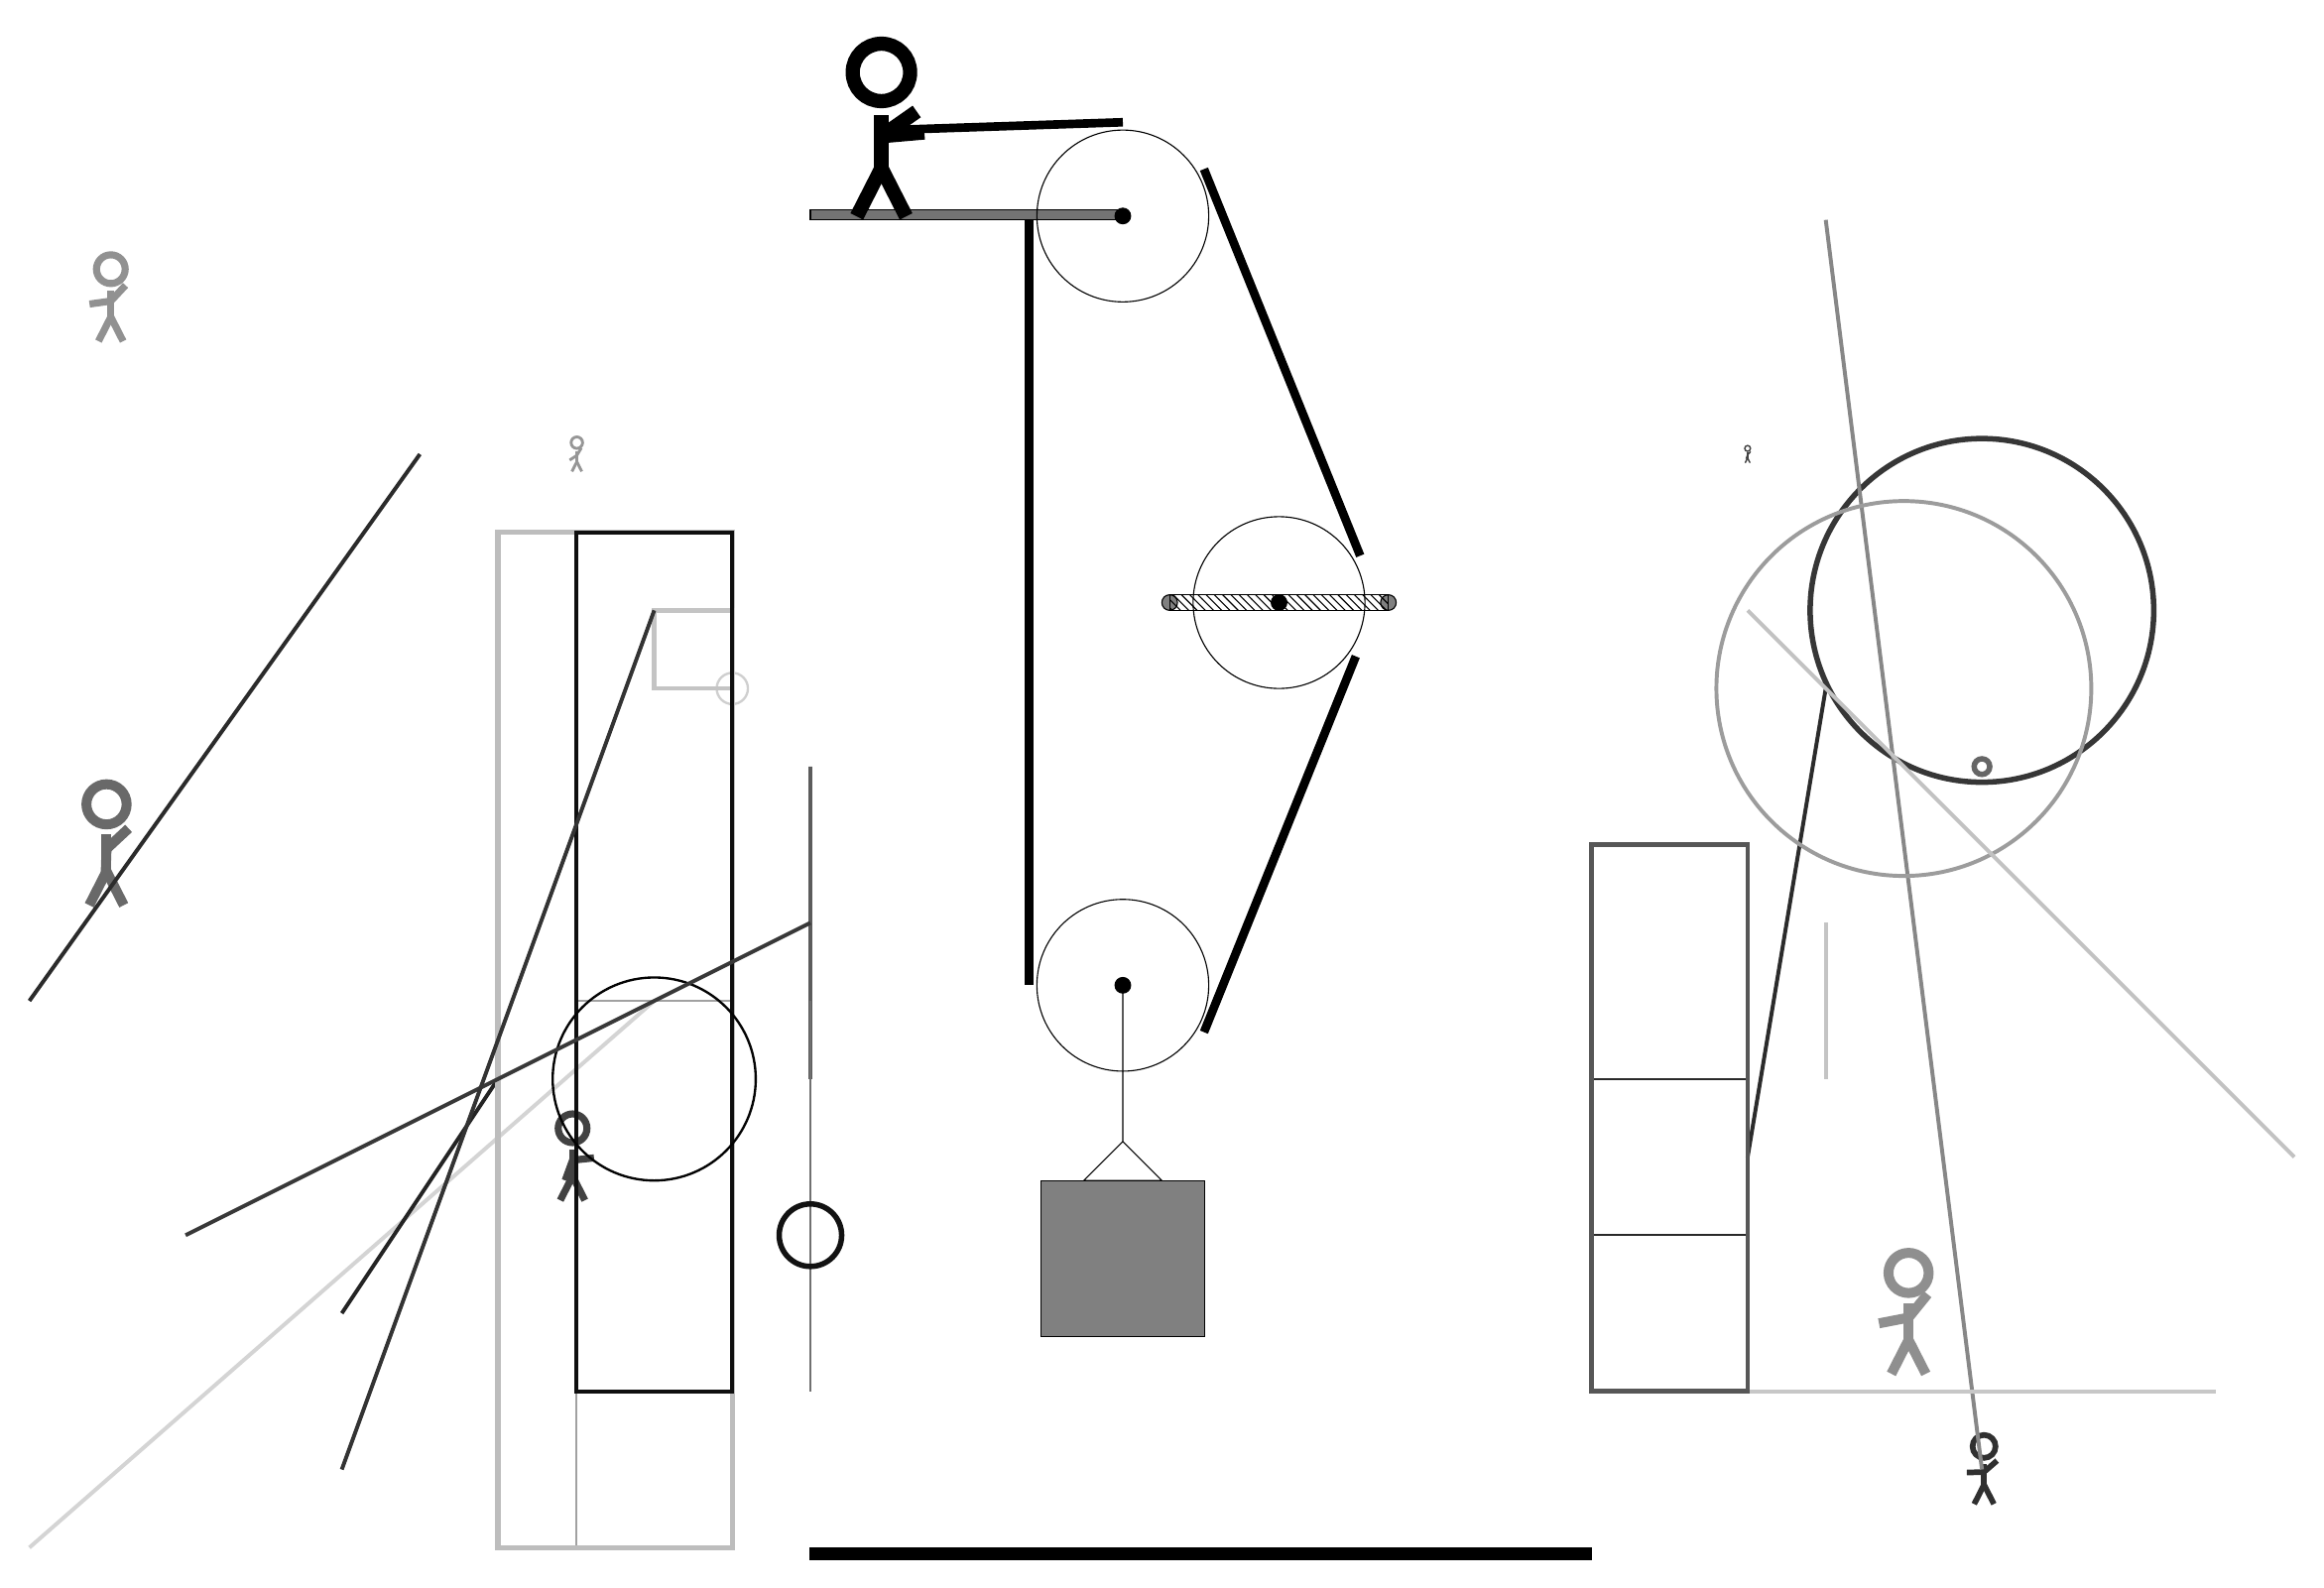
\begin{tikzpicture}
			%%%%% START %%%%%
			
			\draw[fill=black!55] (-2, 14) rectangle (2, 14.125);
			
			\draw (2, 4.2) circle (1.1);
			\draw[fill=black] (2, 4.2) circle (0.1);
			
			\draw (2, 14.05) circle (1.1);
			\draw[fill=black] (2, 14.05) circle (0.1);
			
			\draw[line width=0.3mm, color=black!84] (10, 3) rectangle (8, 1);
			
			\draw [line width=0.7mm, color=black!79](13, 9) circle (2.2);
			\draw[line width=0.4mm, color=black!64] (-2, 3) rectangle (-2, 7);
			\draw[line width=0.5mm, color=black!23](11, 5) -- (11, 3);
			\node[line width=0.2mm, color=black!59] at (-11, 6) {\Strichmaxerl[7][88][43]};
			\draw[line width=0.2mm, color=black!37] (-3, 4) rectangle (-5, -3);
			
			\draw[line width=0.5mm, color=black!83](10, 2) -- (11, 8);
			
			\draw[line width=0.5mm, color=black!17](-4, 4) -- (-12, -3);
			\draw [line width=0.3mm, color=black!19](-3, 8) circle (0.2);
			\node[line width=0.5mm, color=black!74] at (-5, 2) {\Strichmaxerl[5][70][6]};
			\node[line width=0.2mm, color=black!44] at (12, 0) {\Strichmaxerl[7][11][51]};
			\draw[line width=0.5mm, color=black!86](-6, 3) -- (-8, 0);
			\node[line width=0.2mm, color=black!74] at (10, 11) {\Strichmaxerl[1][70][47]};
			\draw[line width=0.7mm, color=black!26] (-3, 10) rectangle (-6, -3);
			\draw[line width=0.6mm, color=black!23] (-3, 8) rectangle (-4, 9);
			\node[line width=0.3mm, color=black!81] at (13, -2) {\Strichmaxerl[4][2][41]};
			
			\draw[line width=0.5mm, color=black!47](13, -2) -- (11, 14);
			\draw[line width=0.5mm, color=black!94] (-3, -1) rectangle (-5, 10);
			\draw [line width=0.3mm, color=black!99](-4, 3) circle (1.3);
			
			\draw [line width=0.5mm, color=black!39](12, 8) circle (2.4);
			\draw[line width=0.5mm, color=black!83](-7, 11) -- (-12, 4);
			\draw[line width=0.5mm, color=black!24](10, 9) -- (17, 2);
			\draw[line width=0.3mm, color=black!56] (-2, -1) rectangle (-2, 4);
			\draw [line width=0.7mm, color=black!60](13, 7) circle (0.1);
			\draw[line width=0.5mm, color=black!22](10, -1) -- (16, -1);
			
			\node[line width=0.7mm, color=black!41] at (-5, 11) {\Strichmaxerl[2][33][59]};
			\node[line width=0.6mm, color=black!43] at (-11, 13) {\Strichmaxerl[5][8][47]};
			\draw[line width=0.5mm, color=black!78](-2, 5) -- (-10, 1);
			\draw[line width=0.6mm, color=black!66] (8, 6) rectangle (10, -1);
			
			\draw[line width=0.5mm, color=black!80](-4, 9) -- (-8, -2);
			\draw [line width=0.7mm, color=black!93](-2, 1) circle (0.4);
			
			
			\draw[fill=white](4, 9.1) circle (1.1);
			\draw[fill=black] (4, 9.1) circle (0.1);
			\draw[fill=black!50] (2.6, 9.1) circle (0.1);
			\draw[fill=black!50] (5.4, 9.1) circle (0.1);
			\draw[pattern=north west lines, pattern color=black] (2.6, 9.2) rectangle (5.4, 9.0);
			
			\draw (2, 4.2) -- (2, 2.2) -- (1.5, 1.7) -- (2.5, 1.7) -- (2, 2.2);
			\draw[fill=black!50] (0.95, 1.7) rectangle (3.05, -0.3);
			
			\draw[line width=1.1mm] (0.8, 14) -- (0.8, 4.2);
			\centerarc[line width=1.1mm](2, 4.2)(180:330:1.2000000000000002);
			\draw[line width=1.1mm](3.0392, 3.6) -- (4.983, 8.4117);
			\centerarc[line width=1.1mm](4, 9.1)(390:325:1.2000000000000002);
			\draw[line width=1.1mm](5.0392, 9.7) -- (3.0392, 14.65);
			\centerarc[line width=1.1mm](2, 14.05)(30:90:1.2000000000000002);
			\draw[line width=1.1mm](2, 15.25) -- (-1, 15.15);
			
			\node at (-1, 15.15) {\Strichmaxerl[10][-175][35]};
			
			\draw[fill=black] (-2, -3) rectangle (8, -3.15);
			
			%%%%% END %%%%%
		\end{tikzpicture}
	\end{figure}	
\end{document}